% declare our document type
\documentclass[12pt]{extarticle}

%%%%%%%% PACKAGES NEEDED FOR THIS DOCUMENT

% allow us to put pictures in the document
\usepackage{graphicx}
% this line lets us use larger fonts
\usepackage{extsizes}
% this allows us to create "slides" in the document
\usepackage[many]{tcolorbox}
% this line lets us caption images inside the "slides"
% this is neccesary since the slide doesn't allow the use of
% \figure{} inside
\usepackage{multicol}
\usepackage{caption}
\usepackage{enumerate}
% allows use of courier font
\usepackage{courier}
% make the table of contents links like people are used to
% the hidelinks parts hides link outlines
\usepackage[hidelinks]{hyperref}
% resize the margins
\usepackage[margin=1in]{geometry}
% use utf8 encoding
\usepackage[utf8]{inputenc}
% one of the other packages complained until I put this here
\usepackage[english]{babel}
% allow citations
\usepackage{cite}
% code listings
\usepackage{listings}
% fix single quote in listings
\usepackage{textcomp}
\usepackage{filecontents}
%\usepackage[noadjust]{cite}
\usepackage{graphicx}
\usepackage{hyperref}
\usepackage{forest,kantlipsum}
\usepackage{float}
\usepackage{etoolbox}
\usepackage{url}
\usepackage{cleveref}
\usepackage{xcolor}
\usepackage[labelfont=bf]{caption}

%%%%%%%%%%% CUSTOM ENVIRONMENT SETUP

% declare a typesetting environment for code/emphasis
\newcommand{\code}[1]{\texttt{\bfseries#1}}
\newenvironment{codeblock}{\bfseries\texttt\bgroup}{\egroup\par}
% better declaration of font environment
%\DeclareTextFontCommand{\codetext}[1]{\code{#1}}
% declare a large font environment for use in the "slides"
\newcommand{\instruction}[1]{\Large{#1}}
% font environment again
%\DeclareTextFontCommand{\instruction}{\instructionfont}
\newenvironment{instructionblock}{\Large\bgroup}{\egroup}

% declare a "slide" text box for use in the document
% the slide is a numbered \section{}
\newtcolorbox[auto counter]{slide}[3][]{%
colback=brown!5!white,colframe=brown!80!gray,height from=4in to 9in,
title={\addcontentsline{toc}{section}{\thetcbcounter ~~ #2}\bf\Large\thetcbcounter ~ #2\hfill #3 \label{slide \thetcbcounter}\setcounter{section}{\thetcbcounter}}}

% declare a "subslide" text box for use in the document
% the subslide is a numbered \subsection{}
\newtcolorbox[auto counter,number within=section]{subslide}[3][]{%
colback=brown!5!white,colframe=brown!80!gray,height from=4in to 9in,
title={\addcontentsline{toc}{subsection}{\thetcbcounter ~~ #2}\bf\Large\thetcbcounter ~ #2\hfill #3 \label{slide \thetcbcounter}}}

\renewcommand{\labelitemii}{$\circ$}

\lstset{basicstyle=\ttfamily,keywordstyle=\bfseries\color{blue!80!black},identifierstyle=\bfseries,stringstyle=\color{red},showstringspaces=false,commentstyle=\itshape\color{green!40!black},upquote=true}

% My Environments (keep these)
\newcommand{\ben}{\begin{enumerate}}
\newcommand{\een}{\end{enumerate}}
\newcommand{\bi}{\begin{itemize}}
\newcommand{\ei}{\end{itemize}}

%%%%%%%%% SET UP OUR TITLE PAGE

\begin{document}
\title{ Firewall Management\\ \normalsize Basic Usage and Configuration of Firewalls in Windows and Ubuntu}
\author{ Ananth Jillepalli \& Risab Manandhar (Versions 1 and 2) \\Gabe Gibler \& Colton Hotchkiss (Version 3) }
\date{July 29, 2017 \\ \hyperref[changelog]{Version 3.4}}
\renewcommand{\abstractname}{Summary}
\begin{titlepage}
\maketitle
\pagenumbering{gobble}
\begin{center}

\includegraphics[scale=.5]{UofI}

\large{CS 439/CS 539: Applied Security Concepts}

\vskip 40pt

\end{center}
\begin{abstract}
A Firewall is a technological barrier which can be used in most computing devices to control the incoming and outgoing network traffic. The controlling is done primarily through use of rules, either pre-configured or user-specified. Effectiveness of firewalls depends upon how well it is managed and not on how perfectly it is deployed. Therefore, in this tutorial, we will demonstrate management (usage and configuration) of firewalls on Windows and Ubuntu operating systems.  
\end{abstract}


\vfill
\begin{center}
	
\includegraphics[scale=0.5]{cc}
	\vskip 10pt
	This work is licensed under a \href{https://creativecommons.org/licenses/by/4.0/}{Creative Commons Attribution 4.0 International License}.
\end{center}

\end{titlepage}

%%%%%%%%%% TABLE OF CONTENTS

\pagebreak
\tableofcontents

%%%%%%%%%%%%%%%%%%%%%%%%%%%%%%%%%%%%%%%%%%%%%%%%%
%%%%%%    BEGINNING OF MAIN BODY OF DOCUMENT
%%%%%%%%%%%%%%%%%%%%%%%%%%%%%%%%%%%%%%%%%%%%%%%%%

\pagebreak
\pagenumbering{arabic}
\setcounter{section}{1}

%----------------------------------------------------------------------------------------------------%





\begin{slide}{ Objectives of this Tutorial }{ \hyperref[slide 2]{\textgreater} }
	\begin{instructionblock}
		\ben
			\item Understand a bit of the history and capabilities of firewalls;
			\item Understand how to manage firewalls through graphical user interfaces (GUI) on Windows and Ubuntu;
			\item Understand the basics of rule-writing to manage firewalls through command line interfaces (CLI);
			\item Apply that knowledge by managing firewalls through both GUI and CLI in a series of activities and challenges.
		\een
	\end{instructionblock}
\end{slide}


\vspace{8mm}
\noindent
This tutorial is not a complete user's guide to firewall management. It is a brief overview of a few firewalls in particular. We will briefly explain, through walkthroughs, activities, and challenges, the following specifics about firewalls:

\ben

\item Firewalls, as we know them today, are a product of a number of transformations from one generation to the next. To truly understand the current state of firewalls, it helps to understand a bit of their history and the course of their development. The capabilities of firewalls are not restricted to the aspects discussed in this tutorial. Most modern firewalls are complex suites of functionality.

\item This tutorial aims to provide a basic understanding of the elements available in a firewall's graphical user interface and how those apply to management of the firewall's functionality.

\item This tutorial also aims to instill a knowledge of the basic usage of the command line interface for writing rules that define network access and other advanced settings within the firewall. 

\item Finally, the skills presented in this tutorial are put to the test by undertaking a set of challenges to provide direct experience of basic firewall management.

\een


%----------------------------------------------------------------------------------------------------%





\pagebreak	
\begin{slide}{ Required Background }{ \hyperref[slide 1]{\textless}\hyperref[slide 3]{\textgreater} }
	\begin{instructionblock}
		We assume some knowledge in the following areas:
		\begin{enumerate}
			\item Experience using computers and software applications, like web browsers, and virtualization apps;
      		\item Fundamentals of internet and networking mechanisms like TCP/IP stack, TCP/UDP protocols and ports, etc.;
			\item An introductory knowledge of data privacy, computer/network security, etc.
		\end{enumerate}
	\end{instructionblock}
\end{slide}


\vspace{8mm}
\noindent
It is not the goal of this tutorial to be completely self-contained and self-explanatory. As such, the tutorial assumes certain background skills and knowledge. The following are some areas where we expect the users of this tutorial to have some previous skills/knowledge:

\ben

\item Practical experience using computers, and installing and using common software applications (particularly web browsers, and virtualization platforms). The tutorial does not always explain how to navigate within the operating system's graphical user interface (GUI) or how to execute commands from the command line. Some exposure to logic notations and elementary programming skills would be very helpful with writing firewall rules. Similarly, the tutorial does not explain how to browse the Internet, or how to install software applications. If setting up the tutorial, additional knowledge is required to set up a domain, set up DNS, etc.

\item Fundamental knowledge of networking mechanisms and computer networks. This tutorial expects a user to understand technical concepts like the ISO OSI model of networks, and common networking terms such as ``packets", ``ports", "protocols", ``accept/drop" in relation to packets, ``TCP" and ``UDP", etc.

\item A broad understanding of general computer-related issues will help, such as ``data privacy", ``network access privileges", ``application permissions", and different sorts of internet-based attacks.

\een 


%----------------------------------------------------------------------------------------------------%





\pagebreak
\begin{slide}{ Hardware and Software Requirements }{ \hyperref[slide 2]{\textless}\hyperref[slide 4]{\textgreater} }
    \begin{instructionblock}
    	The tutorial was executed using the following environment:
    	\begin{enumerate}
    		\item A computer capable of hosting at least 4 virtual machines (VMs);
    		\item A virtualization software platform, e.g. VMWare or VirtualBox;
    		\item A) One standard Microsoft Windows Server 2012 R2 VM, and B) three Ubuntu 15.10 LTS VMs.
    	\end{enumerate}
    \end{instructionblock}
\end{slide}


\vspace{8mm}
\noindent
The activities and challenges of this tutorial occur in multiple VMs. As such, it is imperative that the user of this tutorial has a machine powerful enough to boot at least 4 virtual machines smoothly at a time. For the sake of consistency, specifics for each VM are given below:

\vspace{4mm}
\noindent
\label{WindowsSetup}
\textbf{A}) We are using a standard Microsoft {\textbf{Windows}} Server 2012 R2 VM. You can download it \href{https://www.microsoft.com/en-us/evalcenter/evaluate-windows-server-2012-r2}{\underline{here}} (free 180-day evaluation copy). However, for the Windows Firewall portion of this tutorial, any Windows OS from Windows 7/Windows Server 2008 onwards can be substituted and will be functionally equivalent.

\vspace{4mm}
\noindent
\label{UbuntuSetup}
\textbf{B}) We are using two Ubuntu 15.10 LTS VMs. One should have the package \texttt{gufw} installed. It can be downloaded from the \href{http://gufw.org/}{Gufw Project}. We call this VM \textbf{Ubuntu-gufw}. The other two have the \texttt{LAMP} stack installed. For a guide to installing LAMP on Ubuntu, read this  \href{https://www.digitalocean.com/community/tutorials/how-to-install-linux-apache-mysql-php-lamp-stack-on-ubuntu-16-04}{DigitalOcean {\underline{tutorial}}}. This VM will host a single website with multiple references to it in the Hosts files of the Windows and ``Ubuntu-gufw" VMs. We call it \textbf{Ubuntu-LAMP}. Finally, we also use another VM, which will host any number of websites referenced by the Hosts files of the Windows and ``Ubuntu-gufw" VMs. In addition, it has Nmap installed. We call it either \textbf{Kali} or \textbf{SEED Labs server}, depending which role it serves in a challenge.





%----------------------------------------------------------------------------------------------------%





\pagebreak
\begin{slide}{ Network Layout }{ \hyperref[slide 3]{\textless}\hyperref[slide 5]{\textgreater} }
\vskip 5pt
	\begin{instructionblock}
		\begin{center}
			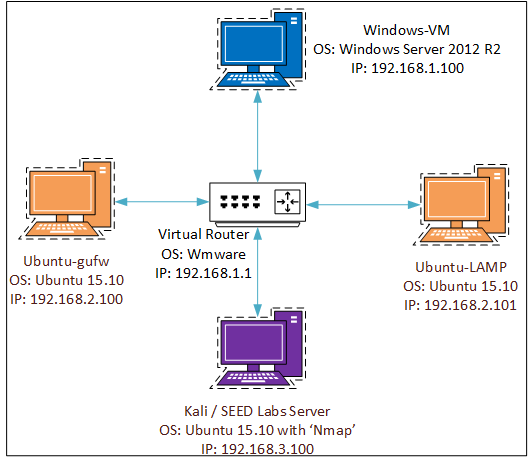
\includegraphics{NetworkDiagram.png}
		\end{center}
	\end{instructionblock}
\end{slide}


%----------------------------------------------------------------------------------------------------%





\pagebreak
\begin{slide}{ A Problem: Network Traffic Control }{ \hyperref[slide 4]{\textless}\hyperref[slide 6]{\textgreater} }
	\begin{instructionblock}
		\ben
			\item { How can system administrators control network traffic and/or network communications originating from or destined to a network address? }
			\item { It requires more than simply monitoring traffic or logging transactions. }
			\item { The process can be complicated at many stages by business and user requirements. A suitable balance between protection, permissions, and allowances is required. }
		\een
	\end{instructionblock}
\end{slide}


\vspace{8mm}
\ben

\item { Controlling network traffic has been an issue since the early days of the internet in the 1980s. Early network traffic control was accomplished by direct router configuration and did not involve any additional software modules or embedded software programs. }

\item { Most confuse traffic controlling with logging the communications or monitoring them because of the overlap of some functionality between the three: controlling, logging, and monitoring. While the latter two might be a subset of the former, depending upon the context of the operation, controlling need not always involve logging and monitoring. }

\item { Network traffic control is an area of conflicting demands, because of the need for users to utilize software and access network and internet resources efficiently and for system administrators to protect important or sensitive resources. A suitable balance between protection, permissions, and allowances must be attained. If protection and permissions are too restrictive, per the concept of least privilege, users become unable to use business software and network resources efficiently. When permissions are broad and protection lax, a greater range of vulnerabilities are made available. }

\een


%----------------------------------------------------------------------------------------------------%





\pagebreak
\begin{slide}{ The Solution: Firewalls }{ \hyperref[slide 5]{\textless}\hyperref[slide 7]{\textgreater} }
\begin{instructionblock}
    \begin{enumerate}
        \item Control of network traffic to and from a computing device;
        \item They are the first line of network protection;
    	\item Different from Intrusion Prevention/Detection Systems(IPS/IDS);
        \item Control program access to a network;
        \item Networks have incoming and outgoing communications. There are often separate rules for both incoming and outgoing traffic.
    \end{enumerate}
\end{instructionblock}
\end{slide}


\vspace{8mm}
\ben
\item { The primary and most significant aspect of Firewalls is to control network traffic to and from a computing device, and the communication media going in and out of a system. Any network security system satisfying the above responsibility can be called a firewall. }

\item { Firewalls are usually the first line of network protection for any given network. Some firewalls, mostly third generation application layer operational level firewall systems, have the ability to functionally perform deep packet inspection. This feature is similar to Intrusion Prevention/Detection, and User Identity Integration. However, the features integrated in the firewalls are not as advanced and should not be used in place of Intrusion Detection/Prevention Systems. }

\item { Modern firewalls also have the ability to configure individual programs or services to be allowed or disallowed, to receive incoming traffic, or send outgoing data. Such a functionality allows for great levels of flexibility in configuring the state of a computing system. Controlling activities naturally involve monitoring and logging of reports, but security systems that only log an monitor are usually not considered firewalls. }

\item { In most firewalls, outgoing communications are allowed by default and incoming traffic is usually filtered. There's a flaw in this approach. If a system is compromised and it can communicate with server, information theft can occur unnoticed and unhampered. Also, if a system is infected and it can communicate with every other system, infectious files can easily propagate to other systems. Thus, outgoing communications should also be filtered at all times. }

\een


%----------------------------------------------------------------------------------------------------%




 
\pagebreak
\begin{slide}{ Classification of Firewalls }{ \hyperref[slide 6]{\textless}\hyperref[slide 8]{\textgreater} }
	\begin{instructionblock}
	    \noindent
		Types of Firewalls:
		\begin{enumerate}
			\item { \textit{Packet-Filtering} (Network Layer); }
			\item { \textit{Stateful Inspection} (Transport/Session Layer); }
			\item { \textit{Application Layer} (Application Layer). }
		\end{enumerate}
        Each item describes a type of functionality, but a firewall may implement multiple types of functionality.
    \end{instructionblock}
\end{slide}


\vspace{8mm}
\ben

\item { \textbf{First Generation:} The first published research on ``firewalls" appeared around 1988, when Digital Equipment Corporation (DEC) developed filter systems known as packet-filtering firewalls. When first introduced, firewalls operated at the network layer in the form of packet filters targeting network addresses and ports of the packet. From that information, the firewall module determined if the packet should be allowed or blocked. }

\item { \textbf{Second Generation:} Dave Presotto, Janardan Sharma, and Kshitij Nigam of AT\&T Bell Laboratories developed the second generation of firewalls and christened them ``circuit-level gateways". In addition to first generation capabilities, second generation firewalls were able to operate at the transport and session layer of the OSI model. Inspection of the ``state" of packets is the distinguishing feature in this generation. It determines whether a packet belongs to a new connection, an existing connection, or a connection that does not exist at all. }

\item { \textbf{Third Generation:} An application suite named \textit{FireWall ToolKit} (FWTK), developed by Wei Xu, Peter Churchyard, and Marcus Ranum, laid the foundations for the next generation of firewalls. The first application layer firewall was an extension of FWTK, enhanced by Wei Xu. The most significant advantage of application layer firewalls is the fact that various protocols are now comprehensible by firewalls and can be included in rule-making. Such protocols include: File Transfer Protocol (FTP), Domain Name System (DNS), and HyperText Transfer Protocol (HTTP). }

\item { Current day firewalls are generally hybrid in nature, because most firewalls have capabilities from packet filtering, stateful inspection, and the application layer.} % Additionally, a few integrate abilities such as serving as proxies and doing network address translation (NAT). }

\een


%----------------------------------------------------------------------------------------------------%





\pagebreak
\begin{slide}{ Locality of Firewalls }{ \hyperref[slide 7]{\textless}\hyperref[slide 9]{\textgreater} }
	%\vskip 10 pt
	\begin{instructionblock}
		\begin{enumerate}
			\item { Firewalls can be situated at different positions within a network and relative to a user:  }
			\begin{enumerate}
				\item { \textit{Endpoint} firewalls, more commonly called \textit{software} firewalls; }
				\item { \textit{Gateway} firewalls, more commonly called \textit{``hardware"} firewalls; }
			\end{enumerate}
			\item { Though location of operation differs, the core functionality is largely all in software;}
			\item { This tutorial utilizes software-based firewalls. }
		\end{enumerate}
	\end{instructionblock}
\end{slide}


\vspace{8mm}
\ben

\item { Firewalls can sit at the point-of-entry for a network, filtering traffic to and from everything on that network, or they can sit at each specific device's connection to a network, filtering traffic for that device alone: }

\ben

\item { \textbf{Software (or Endpoint) firewalls:} This type of firewall operates as software installed on the system it is protecting, and its control extends strictly to the networking interfaces of that system. Software-based firewalls depend heavily on OS support to insert themselves into the network stack. Popular examples of this kind of firewall are: Windows Firewall, Comodo Internet Security, ZoneAlarm, Norton 360, and PeerBlock. }

\item { \textbf{Hardware (or Gateway) firewalls:} These types of firewalls generally operate as firmware on devices dedicated to controlling traffic at entry/exit points for entire local networks. Hardware firewalls can not exercise much control at the application or session layer for any given system on the network. The firewall often co-exists with other network control functionality on its device. Popular examples of this kind of firewall are: Cisco's ASA firewall, Juniper Network's ScreenOS, Dell's SonicWall, and Untangle's Zeroshell. }

\een

\item { Though the location of firewalls differ, they largely all perform the core of their functionality (controlling traffic) in software, rather than as actual circuits in hardware. For this reason, it is actually more appropriate to call ``hardware" firewalls ``firmware" firewalls. Most firewalls of the firmware sort are actually implementations running in a Linux OS on the dedicated ``firewall" device. }

\een


%----------------------------------------------------------------------------------------------------%





\pagebreak
\begin{slide}{ Firewall Limitations }{ \hyperref[slide 8]{\textless}\hyperref[slide 10]{\textgreater} }
\begin{instructionblock}
    \begin{enumerate}
        \item Micromanagement is required for efficient functionality;
        \item Overprotective settings can cripple some applications. If configured to trigger alerts frequently, they can desensitize users to warnings;
        \item Firewalls can be compromised or shut down by other compromised programs;
        \item Firewalls are not a one-stop solution against network attacks. They are not ``defense-in-depth" in \& of themselves.
    \end{enumerate}
\end{instructionblock}
\end{slide}


\vspace{8mm}
\ben

\item { The primary limitation of firewalls is that, for efficient deployment, implementation, and subsequent maintenance, a higher degree of micro-management is required. Micro-management is the term which describes the requirement to specify configurations or policies, with high level of specificity and detail, to a software module or component. The micro-management often makes it tedious for configuring firewalls optimally and many times, system administrators and users just go with either over-zealous and over-protective settings or very lenient settings. }

\item { Both over-protective and lenient firewall settings are not efficient for practical use because in the case of lenient configurations, attack scope increases exponentially. In the case of over-protective settings, apps maybe crippled and if configured to produce alerts, there are many alerts being produced every second that the users of specified system will get desensitized to warnings and will find workaround to firewalls. }

\item { Like any other program, firewalls are not completely immune themselves to vulnerabilities and security flaws, as observed in \textit{Firewalls in News} section. And also, firewalls can be compromised from the inside through another program/service/file which has been compromised through means other than inter-network communication. }

\item { Firewalls provide a fair degree of security protection, but they are not a one-stop solution against network attacks like the Denial of Service attack, the Masquerader attack, and others. Though they are a part of what constitutes a ``defense-in-depth" approach, they are not sufficient by themselves. Still, it is better to have a firewall deployed with minimal configuration, than no firewall at all. }

\een


%----------------------------------------------------------------------------------------------------%





\pagebreak
\begin{slide}{ In the News }{ \hyperref[slide 9]{\textless}\hyperref[slide 11]{\textgreater} }
\begin{instructionblock}
	\begin{enumerate}
		\item Windows Firewall can be bypassed using NBNS.  \\(8th May 2012) \cite{NBNS2012Bojan} [SANS]
		\item IPTables can be bypassed using ``--syn rules". \\(20th June 2014) \cite{CVEDetails2012CVE} [CVE]
		\item Juniper's ScreenOS firewalls possess VPN backdoor. \\(22nd Dec. 2015) \cite{Juniper2015Constantin} [PCWorld]
	\end{enumerate}
\end{instructionblock}
\end{slide}


\vspace{8mm}
\textbf{NOTE:} All of the bypass vulnerabilities discussed below have been patched and are no longer vulnerable on current versions.
\ben

\item { \textbf{Windows Firewall Bypass:} NetBIOS and its weaknesses often pave way for easier medium of spoofing and especially, Name Spoofing. These kind of spoofing attacks were well known since 2005. In the world of Internet today, NetBIOS Name Spoofing have serious impacts on our security. An effective way of preventing this exploit is to not use LM/NT hashes in the Windows systems. In the Domain Controller tutorial, we have discussed on how to disable LM/NT hashes \cite{NBNS2012Bojan}. }

\item { \textbf{IPTables Bypass:} Synchronization rules and Password Synchronization features in IPTables platform using the development switches L2B-05.03.07 and L2E, L2P, L3E, and L3P before 09.0.06 sets an SNMP string to the same string as the administrator password, which allows remote attackers to obtain sensitive information by sniffing the network \cite{CVEDetails2012CVE}. }

\item { \textbf{Juniper's ScreenOS Bypass:} From a mixed cause of likely third party malicious code modifications and Juniper's own cryptography failures, a vulnerability had arisen in Juniper's ScreenOS firewalls which had the potential to allow attackers to decrypt VPN traffic originating from ScreenOS device interfaces. Subsequently, Juniper released patches to address the issue and updated the firmware \cite{Juniper2015Constantin}. }

\een


%----------------------------------------------------------------------------------------------------%





\pagebreak
\begin{slide}{ Quiz: Firewall Background }{ \hyperref[slide 10]{\textless}\hyperref[slide 12]{\textgreater} }
    \begin{instructionblock}
        \bi 
            \item[Q1:] Can Firewalls hinder applications? If so, how does that happen?
            \item[Q2:] What is the difference between a packet filter firewall and an application layer firewall?
            \item[Q3:] ``Defense in depth" is mainly about firewall deployment and management. T/F?
            \item[Q4:] Why are ``hardware" firewalls more properly called ``firmware" firewalls?
        \ei
    \end{instructionblock}
\end{slide}


%----------------------------------------------------------------------------------------------------%





\pagebreak
\begin{slide}{ Firewalls in Windows }{ \hyperref[slide 11]{\textless}\hyperref[slide 13]{\textgreater} }
    \begin{instructionblock}
        \begin{enumerate}
            \item A (very) wide range of private firewall solutions;
            \item For the most part, Microsoft's Windows Firewall is good enough;
            \item Windows Firewall is a GUI-based firewall and packet filter;
        		\ben
        		\item It is a network firewall and an application firewall;
        		\een
            \item Configuration is also available through command-line interface.
        \end{enumerate}
    \end{instructionblock}
\end{slide}


\vspace{8mm}
\ben

\item { Microsoft's Windows operating system, due to its immense popularity, enjoys a wide range of options in many types of applications. Firewalls are not an exception and, as such, there are at least 17 advanced firewall applications in Windows at the time, in active development. Additionally, many commercially successful anti-virus/malware suites have their own integrated firewall. }

\item { For most requirements and everyday configurations, Windows Firewall has intermediate-level features -- not too advanced and not too basic. Windows firewall has an easy-to-use graphical user interface and can mostly be configured using the GUI alone. However, Windows Firewall can be configured by CLI as well. }

\item { By default, Windows Firewall contains three profiles: Domain Network, Private Network, and Public Network. Settings can be customized per profile. }

\een


%----------------------------------------------------------------------------------------------------%





\pagebreak
\begin{slide}{ Activity: Windows Firewall GUI }{ \hyperref[slide 12]{\textless}\hyperref[slide 14]{\textgreater} }
\vskip 5pt
\begin{instructionblock}
The following is for both incoming \& outgoing communications:
\begin{enumerate}
\item Enable/disable firewall.
\item Rule Management:
\subitem Allow/disallow a program/service's network traffic;
\subitem Allow/block a port's network traffic;
\subitem Manage existing rules.
\end{enumerate}
\end{instructionblock}
\end{slide}


\vspace{8mm}
\ben

\item \textbf{To Enable/Disable Windows Firewall:}
\begin{enumerate}
\item Open \textit{Control Panel}.
\item Go to "System and Security" $>$ "Windows Firewall".
\item In the left pane, click on "Turn Windows Firewall on or off".
\item Windows Firewall is turned on or off per profile. (If your computer is not connected to a domain, then you will not see the Domain profile, as is the case with our VM.) 
\item Back in the main \textbf{Windows Firewall} screen, on the left pane, \textbf{Restore Defaults} will reset the entire configuration to factory default.
\end{enumerate}

\item \textbf{Allow/Disallow a Program/Service:}
\begin{enumerate}
\item In the left pane of the main \textit{Windows Firewall} screen, click on "Allow an app or feature through Windows Firewall".
\item Click on "Change Settings".
\item The list of services/programs displayed here are \textbf{Allowed}, which means, it is a white-list.
\item To allow a program/service, click on "Allow another app..." and browse to the location of program/service executable and select it. Before adding this program, click on "Network Types" to select for which profile(s) this rule will be enabled. Finally, click "Add".
\item The profiles for which a rule applies can also be changed using the checkboxes in the \textit{Allowed apps and features} list.
\item To disallow a program/service, select the rule in the \textit{Allowed apps and features} list and click on "Remove".
\end{enumerate}

\item \textbf{Allow/Block a Port:}
\begin{enumerate}
\item In the left pane of the main \textit{Windows Firewall} screen, click on "Advanced Settings". 
\item In the left pane of the new window, select "Inbound Rules" or "Outbound Rules" to create rules for the respective direction of traffic. Either way, the process is similar.
\item In the right pane, click "New Rule...".
\item In the \textit{New Rule Wizard}, select \textit{Port} for the type of rule. Click "Next".
\item Select either \textit{TCP} or \textit{UDP} and specify the range of ports or a single port to allow or block. Click "Next".\\
\hspace{10 mm} \textbf{\texttt{NOTE:} } Allowing all remote ports is NEVER recommended. When blocking, it is at the user's discretion.
\item Select the appropriate option to allow, block, or allow a connection only if it is secure. Once you've made your selection, click "Next".
\item Select any combination of \textit{Domain}, \textit{Private}, or \textit{Public} to choose for which profile(s) the rule will be enforced.
\item Give the rule a name and a description. (Good comments help keep track of the rationale behind a rule when you or someone else come back much later to figure which rules are still valid or not.) Click "Finish" to create the rule.
\end{enumerate}

\item \textbf{Manage Existing Rules:}
\begin{enumerate}
\item In the \textit{Advanced Settings} left pane, select either "Inbound Rules" or "Outbound Rules" again. Rules can be duplicated easily using copy/paste, or removed by pressing \textbf{Delete}.)
\item Creation of a new rule is the same as above. (We created rules for ports, but rules for programs/services or predefined entities can be selected in step \textit{d} above. )
\item  To export or import, in the left pane, click "Windows Firewall with Advanced Security". Importing and exporting options are found in the right pane ("Import Policy..." and "Export Policy...").
\end{enumerate}

\een


%----------------------------------------------------------------------------------------------------%





\pagebreak
\begin{slide}{ Activity: Windows Firewall CLI }{ \hyperref[slide 13]{\textless}\hyperref[slide 15]{\textgreater} }
\vskip 5pt
\begin{instructionblock}
CLI functionality of Windows Firewall can be accessed through Network Shell scripting [netsh]. 
\begin{enumerate}
\item Enable/disable firewall.
\item Rule Management:
\subitem Allow/disallow a program/service traffic;
\subitem Allow/Block a port's network traffic;
\subitem Manage existing rules.
\end{enumerate}
\end{instructionblock}
\end{slide}


\vspace{8mm}
\ben

\item \textbf{To Enable/Disable Windows Firewall (WF):\cite{NetshADV2012Microsoft} }

\begin{enumerate}
\item From the home screen, navigate to the search bar or use \textbf{WIN + S}.
\item Search for \textbf{cmd}. Right-click on \textbf{cmd} and select \textbf{Run as Administrator}.\\
\textbf{\texttt{NOTE} }: This will not work without Admin rights.
\item At the cmd prompt, enter the command:\\
\textbf{\texttt{netsh advfirewall set allprofiles state on} }\\
to enable firewall for all three profiles.

\item Now enter the command:\\
\textbf{\texttt{netsh advfirewall set allprofiles state off} }\\
to disable firewall for all three profiles.

\item Alternative values for \textbf{allprofiles} are:\\
\textbf{currentprofile | domainprofile | privateprofile | publicprofile}

\item To reset the entire WF configuration to factory default, use the command:\\
\textbf{\texttt{ netsh advfirewall reset} }\\

\end{enumerate}

\item \textbf{To Allow/disallow/modify a program/service/port in WF:\cite{NetshADV2012Microsoft}}

\begin{enumerate}

\item To allow a program for all profiles, enter the command:\\
\textbf{\texttt{netsh advfirewall firewall add rule name="AllowProgramMyApp" dir=in action=allow program="C:PATH $\backslash$ filename.extension" \\profile=any enable=yes\\}}
{\textbf{NOTE: } } If bypass is selected and dir=in connecting computers will need to be verified in the rmtcomputergrp along with setting the authentication/encryption flag. If \texttt{dir=out} the authentication/encryption flag must be set.\\


\item The alternative values are as follows: \textbf{\texttt{(dir=in | out), (action=allow | block | bypass), (enable=yes | no), (profile=any | public | \\private | domain)} }

\item To allow a port(i.e. port 655) for all profiles, enter the command:\\
\textbf{\texttt{netsh advfirewall firewall add rule name="AllowPort666" dir=in action=allow protocol=TCP \\ localport=655 profile=any enable=yes} }

\item To disallow a program/service/port, use \textbf{ \texttt{action=block} }. To resolve conflicts, \textbf{\texttt{ action=bypass} } can be used.

\item Deleting a rule(ie. a rule you named Rule43) can be done with the command:\\
\textbf{\texttt{netsh advfirewall firewall delete rule name=Rule43} }
\item Although not recommended, all rules can be deleted with the command:\\
\textbf{\texttt{netsh advfirewall firewall delete rule all} }

\item To modify an existing rule(i.e. a rule named AllowMessenger) to require a new security type, use the command:\\
\textbf{\texttt{set rule name="AllowMessenger" new security=authenticate} }
\textbf{NOTE:} The keyword "new" is placed before the parameter you are changing.

\item Example commands can be found with:\\
\textbf{\texttt{netsh advfirewall firewall add rule ?} }

\item Existing rules can be scanned using command:\\
\textbf{\texttt{netsh advfirewall firewall show rule name=all profile=any} }.\\ This list can be very large and you may just want to view a specific rule with the command:\\
\textbf{\texttt{ netsh advfirewall firewall show rule name=RName } }\\
where "RName" is the name of the rule you would like to view.

\item To Export your policy use the command:\\
\textbf{\texttt{netsh advfirewall export "PATH $\backslash$ filename.wfw"} }
\item To Import a policy use the command:\\
\textbf{\texttt{netsh advfirewall import "PATH $\backslash$ filename.wfw"} }
\end{enumerate}

\een

%----------------------------------------------------------------------------------------------------%





\pagebreak
\begin{slide}{ Challenge 1: Windows Firewalls }{ \hyperref[slide 14]{\textless}\hyperref[slide 16]{\textgreater} }
\vskip 5pt
\begin{instructionblock}
	Use the ``Windows Server 2012" and Kali VMs to perform the following tasks:
	\begin{enumerate}
	\item { Disable Windows Firewall; }
	\item { From the Kali VM, scan the Windows Server machine to see how it appears from an outside perspective. What ports are open? What other info can be gathered? }
	\item Now Enable Windows Firewall and perform the scan again. What are the differences?
	\end{enumerate}
	
	\textbf{\Large{Deliverables:}}
	\ben
		\item Observations of the differences in scanning outcomes with the firewall enabled and disabled.
	\een

  \vspace{20mm}
  \begin{center}
  \textbf{\Large{Duration: 8 min.} }
  \end{center}
\end{instructionblock}
\end{slide}


\vspace{8mm}
\noindent


%----------------------------------------------------------------------------------------------------%





\pagebreak
\begin{slide}{ Challenge 2: Windows Firewalls }{ \hyperref[slide 15]{\textless}\hyperref[slide 17]{\textgreater} }
	\vskip 5pt
\begin{instructionblock}
	Using GUI, block Remote Desktop Connection for all IP addresses: 
	\begin{enumerate}
	\item Block it for all three firewall profiles;
	\item Block it both incoming and outgoing.
	\end{enumerate}
	
	Create an exception for an IP address or an entire subnet of IP addresses. For example, the subnet 192.168.1.100/24.
	
\end{instructionblock}
\textbf{\Large{Deliverables:}}
\ben
\item Remote Desktop should be blocked in all cases except for the specified IP addresses.
\een

\vspace{20mm}
\begin{center}
	\textbf{\Large{Duration: 20 min.} }
\end{center}

\end{slide}  


\vspace{8mm}
\noindent
\textbf{HINTS:}\\
For effective implementation, both programs and services must be customized while defining rules. Source executable of \textit{Remote Desktop Connection} can be found by examining the \texttt{Open file location} option of RDP properties. Rules can be modified when and as needed.


%----------------------------------------------------------------------------------------------------%





\pagebreak
\begin{slide}{ Challenge 3: Windows Firewalls }{ \hyperref[slide 16]{\textless}\hyperref[slide 18]{\textgreater} }
\vskip 5pt
\begin{instructionblock}
	Use Windows Firewall to perform the following tasks:
	\begin{enumerate}
	\item{ Add a rule to block problematic typosquatter website(s) that are continual sources of malware on your network. Test that the bad websites are blocked, but that you can still navigate normally to other websites. }
	\end{enumerate}

\end{instructionblock}
\textbf{\Large{Deliverables:}}
\ben
\item Only the problematic websites should be blocked; all others should still be accessible.
\een

\vspace{20mm}
\begin{center}
	\textbf{\Large{Duration: 10 min.} }
\end{center}
\end{slide}


\vspace{8mm}
\noindent
\textbf{HINTS:}
\begin{enumerate}

\item[2.] The typosquatter websites are \textbf{facbook.com}, \textbf{gogle.com}, and \textbf{mikrosoft.com}. They are all hosted on the ``Ubuntu-LAMP" server.

The regular websites to test against are hosted on the SEED Labs server. They are \textbf{wtmobilestore.com}, \textbf{wtelectronicsstore.com}, \textbf{wtcamerastore.com} and \textbf{wtshoestore.com}.

To find the IP address for a domain name, you can use the \texttt{nslookup} command.

\end{enumerate}



%----------------------------------------------------------------------------------------------------%





\pagebreak
\begin{slide}{ Firewalls in Linux }{ \hyperref[slide 17]{\textless}\hyperref[slide 19]{\textgreater} }
\vskip 5pt
\begin{instructionblock}
\begin{enumerate}
\item Linux is relatively command-line oriented; subsequently so are its firewalls;
\item \texttt{gufw} and \texttt{iptables} (previously \texttt{ipchains}) are examples of software firewalls for Linux;
\item \texttt{gufw} (GUI for Uncomplicated FireWall) is an easy-to-use front-end for a command-line interface (CLI) firewall, \texttt{ufw};
\item \texttt{iptables} is a fairly advanced firewall with many integrated tools like user-space administration, packet filtering, protocol filters, and network filters.
\end{enumerate}
\end{instructionblock}
\end{slide}


\vspace{8mm}
\ben

\item { Most Linux firewalls have a highly advanced and flexible command set for command-line interface (CLI). }

\item { For everyday uses, Ubuntu has \texttt{gufw} (GUI Uncomplicated FireWall). \texttt{gufw} is a front-end for \texttt{ufw}. It has an easy-to-use graphical interface, and can generally be configured through the GUI. If command-line is more your style, \texttt{iptables} is available and active in Linux kernel by default. It is entirely CLI. \texttt{ufw} is also available. It is derived from \texttt{iptables} and may be an easier option. }

\item { \texttt{gufw} by default contains three profiles: Home Network, Public Network, and Office Network. Configurations and settings can be customized per profile. 

\item \texttt{iptables}' methodology is called ``chains". They are configured as linked chains of rules. }

\een


%----------------------------------------------------------------------------------------------------%





\pagebreak
\begin{slide}{ Activity: gufw }{ \hyperref[slide 18]{\textless}\hyperref[slide 20]{\textgreater} }
\vskip 5pt
\begin{instructionblock}
\begin{enumerate}
\item Basic Functionality:
\bi
\item Setting preferences, managing profiles, enabling/disabling profiles, and controlling traffic.
\ei
\item Rule Management:
\bi
\item Adding, editing and removing rules.
\ei
\item Dynamic Rule Generation:
\bi
\item Creating/editing rules dynamically from reports.
\ei
\end{enumerate}
\end{instructionblock}
\end{slide}


\vspace{8mm}
\ben

\item \textbf{Basic Functionality:}

\begin{enumerate}

\item Open \texttt{gufw}: \textbf{System Settings} $>$ \textbf{System}, "Firewall Configuration".

\item In the top menu, go to \textbf{Edit} $>$ \textbf{Preferences}.

\item In the dialog box, change "Logging" to \textit{Full}. 

\item Check the boxes for "Logging Gufw activity" and "Show confirm dialog box for deleting rules". 

\item Adjust the Listening Report's "Refresh Interval" to \textit{1"}.

\item In the \textbf{Profiles} section, there are three profiles by default: Office, Public and Home. Currently we have Home and Lab. Any profile except the current one can be deleted. A total of 255 profiles can be created. To create profiles, use the \textbf{+} symbol. To delete, use the \textbf{-} symbol. Profiles can be renamed by double-clicking their name. A profile's name may be a maximum of 15 characters. 

\item Enabling or disabling \textit{Gufw} is done per profile. Select a profile. Toggle the "Status" button \textit{ON} or \textit{OFF}, and the firewall will be enabled or disabled respectively while using that profile.

\item Controlling global traffic is done per profile, as well. Select a profile and set values in the "Incoming" and "Outgoing" drop-downs. \textit{Allow} permits all communications for that channel. \textit{Deny} drops all communication for that channel. \textit{Reject} drops all communications as well, but also sends a message to the computer on the other end of the connection that their communication attempts have been rejected.
\end{enumerate}

\item \textbf{Rule Management:}

On the main window, the \textbf{Rules} section can be used to create custom rules. Once again the \textbf{+} and \texttt{-} symbols are used to add and delete rules. 

In the "Add a Firewall Rule" window, there are three tabs.

\begin{enumerate}

\item The ``Preconfigured" tab offers easy configuration for specific applications. The list of applications can be filtered by \textit{Category} and \textit{Subcategory}. 

\item The ``Simple" tab allows configuration of specific port and transport protocol combinations for incoming and outgoing traffic.

\item The ``Advanced" tab contains options that enable the creation of completely customized rules. New options presented here are \textbf{Interface}, \textbf{Logging Flexibility}, and \textbf{Custom IP Addresses and Ports}. The \textbf{Interface} tab is for the creation of rules for specific interfaces available to the system. For \textbf{Logging Flexibility}, it is always recommended to \textit{Log All}. Last but not least, a custom range of ports and IP addresses can be used to design highly specific firewall rules.\\\\The ``Policy" field presents a new option, \textit{Limit}. \textit{Limit} will deny connections from an IP address if it attempts to connect more than 5 times within a 30 second time frame.

\end{enumerate}


\item \textbf{Dynamic Rule Generation}

\begin{enumerate}

\item On the main window, \textbf{Report} lists ports that are actively listening. This feature is not very effective for assisting with attack prevention, since it only generates information about active ports. But, it is very helpful for thwarting continuous, repeated exploit attempts. 

\item Firewall rules can be added dynamically from \textbf{Report}. Click a port in the list, then click the \textbf{+} button. This jumps to a new rule in the \textbf{Advanced} tab with many details filled in automatically for you, matching the rule you selected.
\end{enumerate}

\een


%----------------------------------------------------------------------------------------------------%





\pagebreak
\begin{slide}{ Activity: iptables }{ \hyperref[slide 19]{\textless}\hyperref[slide 21]{\textgreater} }
\vskip 5pt
\begin{instructionblock} 
\begin{enumerate}
\item Basic Functionality:
\bi
\item Enabling/disabling, checking status, and logging
\ei
\item Chain Management:
\bi
\item Adding, editing and removing chains.
\ei
\item Rule Management:
\bi
\item Adding, editing and removing rules.
\ei
\end{enumerate}
\end{instructionblock}
\end{slide}


\vspace{8mm}
\ben

\item \textbf{Basic Functionality:}

\begin{enumerate}

\item To check what rules are in effect, try either of the following commands and their various options:

\texttt{\textbf{sudo iptables -L[ chain-name|TCP|UDP][ -v]}}

\texttt{\textbf{sudo iptables -S[ chain-name|TCP|UDP]}}

Rules are grouped according to chain. The columns displayed for each rule: \textbf{target}, \textbf{prot}(ocol), \textbf{opt}(ions), \textbf{source}, \textbf{destination} and \textbf{notes}.

\item It is not necessary to log all traffic in and out of a firewall. Doing so can create very large log files. It is more practical to only log dropped packets. That can be set using the following command:

\texttt{\textbf{sudo iptables -I INPUT -j LOG --log-prefix "iptables denied: " --log-level 7}}

Logs are saved at \textit{/var/log/syslog}. There are seven levels of logging:

\begin{center}
\begin{tabular}{ |c|c| } 
 \hline
Level Number &  Meaning \\
 \hline
0  &     Emergency: system is unusable \\
1  &     Alert: action must be taken immediately \\
2  &     Critical: critical conditions \\
3  &     Error: error conditions \\
4  &     Warning: warning conditions \\
5  &     Notice: normal but significant condition \\
6  &     Informational: informational messages \\
7  &     Debug: debug-level messages \\
 \hline
\end{tabular}
\end{center}

\item To save all changes, so they remain the next time the \texttt{iptables} service is restarted, you must use the following command (on Ubuntu):

\texttt{\textbf{sudo /sbin/iptables-save}}

\item \texttt{iptables} is enabled by default in Linux, and is integrated at the kernel level. There's no real way to turn it on or off. One can fully configure all settings as desired, and save the configuration file. Then, use a command to flush every rule, set the default chains to accept all traffic, configure any necessary routing or services for basic network functionality, and save that configuration file separately. Then, switch back and forth between the config files to not lose the original settings. 

The flush command is:

\texttt{\textbf{sudo iptables -F}}

\end{enumerate}


\item \textbf{Chain Management:}
\begin{enumerate}

\item \texttt{iptables} has three chain types by default. They are: \textit{INPUT}, \textit{FORWARD}, and \textit{OUTPUT}. The \textit{INPUT} chain is for processing incoming connections. The \textit{OUTPUT} chain is for processing connections originating from your own computer. The \textit{FORWARD} chain is for processing connections that are only being forwarded and are not intended for this computer itself. This chain is not generally used. 

To create more chains, use the command: 

\texttt{\textbf{iptables -N chain-name}}

\item When a request does not match any rules in a chain, \texttt{iptables} has default policies to handle it. The default policies can be set to either accept or drop.

\texttt{\textbf{iptables --policy INPUT ACCEPT|DROP}}\\
\texttt{\textbf{iptables --policy OUTPUT ACCEPT|DROP}}\\
\texttt{\textbf{iptables --policy FORWARD ACCEPT|DROP}}

\item To list the rules present in a chain, use the command: 

\texttt{\textbf{iptables -L chain-name}}

\item To flush a chain of all rules, use the command:

\texttt{\textbf{iptables -F chain-name}}

\item To rename a chain, use the command: 

\texttt{\textbf{iptables -E old-chain-name new-chain-name}}

\item To delete a chain, use the command:

\texttt{\textbf{iptables -X chain-name}}

Root privileges are required to delete one of the three default chains. 

\end{enumerate}


\item \textbf{Rule Management:}
\begin{enumerate}

\item To add rules to a chain, use the following command syntax:

\texttt{\textbf{sudo iptables -A chain-name[ -s \{IP Address|hostname\}][ -d \{IP Address|hostname\}][ -p tcp|udp ] -j ACCEPT|DROP|REJECT\\|LOG|chain-name}}

\texttt{-A} specifies the instruction to append a rule to a chain.\\
\texttt{-s} specifies a source IP address or name to match.\\
\texttt{-d} specifies a destination IP address or name to match.\\ \texttt{-p} specifies a protocol to target.\\
\texttt{-j} specifies what to do when the rule is processed, including jumping to other chains for processing.\\
There are also \texttt{-sport} and \texttt{-dport} options to specify source and destination ports \cite{IPTablesSPortDPort}.

An interesting extra: \texttt{!} can be used as a "not" operator with -s and -d.

These and numerous other options are available for -A and the other commands that follow.

\item Instead of \texttt{-A} to append the rule to the end of a chain, \texttt{-I} inserts a rule at a specific position within a chain. For example, to insert a rule at the 4th position in a chain:

\texttt{\textbf{sudo iptables -I chain-name 4}}

\item \texttt{-R} specifies the position of an existing rule to replace. For example, to replace the 4th rule in a chain:

\texttt{\textbf{sudo iptables -R chain-name 4}}

\item To delete a rule from any chain, use \texttt{-D}. There are two ways a rule can be deleted using this option. If we provide a rule position number, then the rule at that particular position will be deleted from the chain. If no rule number is provided, then the first rule matching the given options is deleted. The rul must be an exact match, though. For example, to delete the rule at the 4th position in a chain:

\texttt{\textbf{sudo iptables -D chain-name 4}}

To delete the first rule permitting UDP traffic:

\texttt{\textbf{sudo iptables -D chain-name -p udp -j ACCEPT}} 

\end{enumerate}

\een


%----------------------------------------------------------------------------------------------------%





\pagebreak
\begin{slide}{ Challenge 4.a: Linux Firewalls }{ \hyperref[slide 20]{\textless}\hyperref[slide 22]{\textgreater} }
\vskip 5pt
\begin{instructionblock}
	Use the ``Ubuntu-GUFW" and Kali VMs to perform the following tasks:
	\begin{enumerate}
	\item { Disable both firewalls; }
	\item { From the Kali VM, scan the Ubuntu VM to see how it appears from an outside perspective. What ports are open? What other info can be gathered? }
	\end{enumerate}

\end{instructionblock}

\textbf{\Large{Deliverables:}}
\ben
\item Observation of what is visible from outside when the firewalls are disabled.
\een

\vspace{20mm}
\begin{center}
	\textbf{\Large{Duration: 10 min.} }
\end{center}

\end{slide}


\vspace{8mm}
\noindent
\textbf{HINTS:}
\begin{enumerate}

\item When disabling the firewalls, we need to disable both. But because \texttt{iptables} is configured at the kernel level, one does not simply disable \textit{iptables}. Make it as passive as possible on all chains.

\end{enumerate}


%----------------------------------------------------------------------------------------------------%





\pagebreak
\begin{slide}{ Challenge 4.b: Linux Firewalls }{ \hyperref[slide 21]{\textless}\hyperref[slide 23]{\textgreater} }
\vskip 5pt
\begin{instructionblock}
	(Continued from the previous task.)
	\begin{enumerate}
	\item[3] { Enable \texttt{gufw}, leaving \texttt{iptables} as-is. Set ``Incoming" to \textit{Deny}, if not already so; }
	\item[4] { Repeat the scans from the Kali VM. What differences do you see? }
	\item[5] { Disable \texttt{gufw}, and set the default chains in \texttt{iptables} to \texttt{DROP}. }
	\item[6] { Scan again from the Kali VM. Any differences? }
	\end{enumerate}

\end{instructionblock}

\textbf{\Large{Deliverables:}}
\ben
\item Observation of what is visible from outside when the firewalls are enabled in turn individually.
\een

\vspace{20mm}
\begin{center}
	\textbf{\Large{Duration: 15 min.} }
\end{center}

\end{slide}


%\vspace{8mm}
%\noindent
%\textbf{HINTS:}
%\begin{enumerate}
%
%\item 
%
%\end{enumerate}


%----------------------------------------------------------------------------------------------------%





\pagebreak
\begin{slide}{ Challenge 5: gufw }{ \hyperref[slide 22]{\textless}\hyperref[slide 24]{\textgreater} }
\vskip 5pt
\begin{instructionblock}
	On the ``Ubuntu-GUFW" VM, use \texttt{gufw} to perform the following tasks:
	\begin{enumerate}
	\item{ Block and log all traffic related to Steam and send a message to the person attempting communication, conveying the block; }
	\item{ Add a rule to block problematic typosquatter website(s) that are continual sources of malware on your network. Test that the bad websites are blocked, but that you can still navigate normally to other websites. Remove the rule. }
	\end{enumerate}

\end{instructionblock}

\textbf{\Large{Deliverables:}}
\ben
\item Any usage of Steam should be rejected (versus simply dropped);
\item Only the problematic websites should be blocked; all others should still be accessible. 
\een

\vspace{20mm}
\begin{center}
	\textbf{\Large{Duration: 15 min.} }
\end{center}

\end{slide}


\vspace{8mm}
\noindent
\textbf{HINTS:}
\begin{enumerate}

\item The typosquatter websites are \textbf{facbook.com}, \textbf{gogle.com}, and \textbf{mikrosoft.com}. They are all hosted on the ``Ubuntu-LAMP" server.

The regular websites to test against are hosted on the SEED Labs server. They are \textbf{wtmobilestore.com}, \textbf{wtelectronicsstore.com}, \textbf{wtcamerastore.com} and \textbf{wtshoestore.com}.

To find the IP address for a domain name, you can use the \texttt{nslookup} command.

\end{enumerate}


%----------------------------------------------------------------------------------------------------%





\pagebreak
\begin{slide}{ Challenge 6: iptables }{ \hyperref[slide 23]{\textless}\hyperref[slide 25]{\textgreater} }
\vskip 5pt
\begin{instructionblock}
	On the ``Ubuntu-GUFW" VM, use \texttt{iptables} to perform the following tasks:
	\begin{enumerate}
	\item{ Write two rules to block pings. Test your rules to make sure they work. Then, remove them; }
	\item{ Add a rule to block problematic typosquatter website(s) that are continually sources of malware on your network. Test that the bad websites are blocked, but that you can still navigate normally to other websites. Remove the rule. }
	\end{enumerate}

\end{instructionblock}

\textbf{\Large{Deliverables:}}
\ben
\item Pings to ``Ubuntu-GUFW" should be unresponsive; 
\item Only the problematic websites should be blocked; all others should still be accessible. 
\een

\vspace{20mm}
\begin{center}
	\textbf{\Large{Duration: 15 min.} }
\end{center}

\end{slide}


\vspace{8mm}
\noindent
\textbf{HINTS:}
\begin{enumerate}

\item Two rules are needed, one for the \textit{INPUT} chain and the other for \textit{OUTPUT}.   

\item See the \texttt{gufw} challenge above for the websites to test against.

\texttt{iptables} can block by either IP address or domain name.

\end{enumerate}


%----------------------------------------------------------------------------------------------------%





\pagebreak
\begin{slide}{ Bonus Challenge: Windows Firewall GPO }{ \hyperref[slide 24]{\textless}\hyperref[slide 26]{\textgreater} }
\vskip 5pt
\begin{instructionblock}
	Windows Firewall can be configured up to an extent through Microsoft's Group Policy Editor. For domain profile, do the following:
	\begin{enumerate}
	\item Disable \texttt{local program exceptions};
	\item Disable \texttt{prohibit notifications};
	\item Enable \texttt{logging dropped packets};
	\item Disable \texttt{local ports exceptions}.
	\end{enumerate}

\end{instructionblock}

\textbf{\Large{Deliverables:}}
\ben
\item Client machines should be unable to specify any local program exceptions contrary to Windows Firewall policies set by Domain Controller.
\item Windows Firewall should no longer notify when it is in a critically insecure state.
\item Dropped packets should be logged and viewable in Windows Event Viewer.
\item Client machines should be unable to specify local exceptions for ports contrary to Windows Firewall policies set by Domain Controller.
\een

\vspace{20mm}
\begin{center}
	\textbf{\Large{Duration: 30-45 min.} }
\end{center}

\end{slide}


\vspace{8mm}
\noindent
\textbf{HINT:} Firewall settings are a component of network connections to be used as a part of an overall network for deploying administrative templates of computer configuration.


%----------------------------------------------------------------------------------------------------%





% bibliography on last page
\pagebreak
\begin{slide}{ Conclusion }{ \hyperref[slide 25]{\textless}\hyperref[slide 27]{\textgreater} }
	\begin{instructionblock}
		\begin{enumerate}
			\item There are many types of firewalls to choose from. Despite the variety, their core functionality is similar;
			\item Firewalls are easy to install and access, but can be relatively difficult to configure for optimal functionality;
			\item Through these walkthroughs and hands-on activities, we've learned some basic management of firewalls in Windows and Linux.
		\end{enumerate}
	\end{instructionblock}
\end{slide}


\vspace{8mm}
\begin{enumerate}
\item { There are many software firewalls to choose from. Some of them offer easy to use graphical user interfaces, like \texttt{gufw}, some are very sophisticated to use, like \texttt{iptables}, and some are flexible to accommodate both ease of use and sophisticated rule management, like \texttt{Windows Firewall}. 

Despite the variety, the core functionality of every firewall remains the same: to place the management of network traffic in the user's control. }
\item { Unlike service applications which are easier to maintain and configure, firewalls are relatively difficult in nature to maintain and configure for optimal functionality. Setup of a firewall is very trivial in most cases, but the ensuing configuration can take a long time depending on an organization's needs. }
\item { In this tutorial, we have seen how \texttt{Windows Firewall} works (both GUI and CLI), and we have seen examples of Ubuntu firewalls with \texttt{gufw} and \texttt{iptables}. }

\end{enumerate}


%----------------------------------------------------------------------------------------------------%





\pagebreak	
\begin{slide}{ Appendix: Solutions and Change Log }{ \hyperref[slide 26]{\textless} }
	\begin{instructionblock}
		\begin{enumerate}
			\item Answers to the Quiz;
			\item Solutions to the Challenges:
      \ben
				\item Challenge 1;
				\item Challenge 2;
				\item Challenge 3;
				\item Challenge 4;
				\item Challenge 5;
				\item Challenge 6;
				\item Bonus Challenge;
			\een
			\item Change Log.
		\end{enumerate}
	\end{instructionblock}
\end{slide}



\newpage
\textbf{Answers to the Quiz:}	

\ben

\item Over-protective configurations can cause major hindrances to some applications, effectively crippling them. 

\item Packet filter firewalls are able to control traffic related to ports, IP addresses and network requests. Application layer firewalls can do all that and in addition, can configure rules with respect to specific applications and services.

\item ``Defense in depth" approach is not about just firewalls. There are many layers of protection. Firewalls are often the first line of protection for a network. 

\item They are more properly called ``firmware" firewalls because most firewalls carry out their duties at the software level as applications in Linux, rather than as actual circuits in hardware.

\een


\newpage
\textbf{Solutions to the Challenges:}	

\ben

\item \textbf{Challenge 1:}
\begin{enumerate}
\item In ``Inbound Rules" section, click on ``New Rule" at the right pane. 
\item In resultant wizard, Custom Rule type. All Programs.
\item Protocol type: ICMPv4. Scope: Any IP address.
\item Action: Block the connection. Profile: All three.
\item Give a RULENAME and description. Then, finish.
\item Repeat the same by changing Protocol type to ICMPv6.
\item Repeat the same thing twice (once for ICMPv4 and another for ICMPv6) in ``Outbound Rules".  
\end{enumerate}

\noindent
To disable rules using CLI, use the command: \texttt{netsh advfirewall firewall set rule name="RULENAME" new enable=no}, where RULENAME is the name of rule which one has assigned at the end of creating every rule. 
 

\vspace{4mm}
\item \textbf{Challenge 2:}
\begin{enumerate}
\item In ``Inbound Rules" section, click on ``New Rule" at the right pane. 
\item In resultant wizard, Custom Rule type. 
\item Program: The program path is: \texttt{C-Windows-System32-mstsc.exe}.
\item Services: \textit{Customize}. Apply to all services beginning with the name ``Remote Desktop Services".
\item Any protocol type -- Any IP addresses -- Block the connection-All Profiles
\item Give a name and description. Then, finish.
\item Repeat the same for ``Outbound Rules".
\end{enumerate}

\noindent
To create an exception for 192.168.1.100/24 subnet, 

\begin{enumerate}
\item In ``Inbound Rules" section, right click on the rule created in PART-1 of the challenge.  
\item Go to \texttt{General} tab. Change \textit{Action} from \texttt{Block the connection} to \textit{Allow the connection}.
\item Go to \texttt{Scope} tab. Do the following step for both \texttt{Local IP address} and \texttt{Remote IP address}
\item Change radio selection to \texttt{These IP addresses:}. Click on button \texttt{Add} and enter the subnet value \texttt{192.168.1.100/24}
\item Apply the modifications and \texttt{OK} to change the rule.
\item Repeat the same for ``Outbound Rules".
\end{enumerate}


\vspace{4mm}
\item \textbf{Challenge 3:}
\begin{enumerate}
\item To block the offending website(s), you will need an IP address. In command prompt execute the following command:\\
\texttt{\textbf{nslookup {websitename} } }
\item In the Windows Firewall Advanced Settings:

  Create an inbound and outbound rule as follows:
	\ben
    \item Select \texttt{"New Rule"}
    \item Select \texttt{"All Programs"}
    \item Protocol type \texttt{Any} and \texttt{All Ports}
    \item Under \texttt{"Which remote IP addresses does this rule apply to?" }
    \item Add the IP address of the offending website and select \texttt{"Next"}.
    \item Select \texttt{"Block the connection"}
    \item Select for all profiles.
    \item Name the rule.
  \een
\item Now test to make sure your rule works
\end{enumerate}


\vspace{4mm}
\item \textbf{Challenge 4:}\\
\begin{enumerate}
\item \ben
        \item In \texttt{gufw}, switch the state of the current profile to \textit{OFF}.
        \item Open a terminal.
        \item Execute the following 3 commands to make sure each of the default chains in \texttt{iptables} are set to \texttt{ACCEPT}:
        
        \texttt{\textbf{sudo iptables --policy INPUT ACCEPT}}

        \texttt{\textbf{sudo iptables --policy OUTPUT ACCEPT}}

        \texttt{\textbf{sudo iptables --policy FORWARD ACCEPT}}
        
        \item You might execute the following commands to confirm each chain states ``Chain \{chain-name\} (policy ACCEPT)":
        
        \texttt{\textbf{sudo iptables -L}}
        
        OR
        
        \texttt{\textbf{sudo iptables -L INPUT}}
        
        \texttt{\textbf{sudo iptables -L OUTPUT}}
        
        \texttt{\textbf{sudo iptables -L FORWARD}}
        
    \een
\item On the Kali VM:
    \ben
        \item Open a terminal.
        \item Initially, execute the following command to see if you can determine the IP address of the target machine (``Ubuntu-gufw"):
        
        \texttt{\textbf{nmap 192.168.1.0/24}}
        
        \item Once you have the IP address, execute the following command:

        \texttt{\textbf{nmap -p "*" \{IP Address\} -sV -sS -O -T4}}
        
        \item What you see is that Nmap reports all ports as closed, and the OS could not be identified.
    \een

\item Return to the ``Ubuntu-GUFW":
    \ben
        \item In \texttt{gufw}, switch status to \textit{ON}.
        \item Set ``Incoming" to \textit{DENY}, if it is not already set to that.
    \een

\item Repeat step 2. Nmap reports that all ports are now filtered. The OS is still not recognizable.

\item Return to the ``Ubuntu-GUFW":
    \ben
        \item In \texttt{gufw}, switch the state of the current profile to \textit{OFF}.
        \item In the terminal, execute the following commands:
        
        \texttt{\textbf{sudo iptables --policy INPUT DROP}}

        \texttt{\textbf{sudo iptables --policy OUTPUT DROP}}

        \texttt{\textbf{sudo iptables --policy FORWARD DROP}}
        
    \een
    
\item Repeat step 2. Nmap still reports that all ports are filtered, the OS indeterminate.

\item Before continuing, set \texttt{iptables} back to an open state:
        
\texttt{\textbf{sudo iptables --policy INPUT ACCEPT}}

\texttt{\textbf{sudo iptables --policy OUTPUT ACCEPT}}

\texttt{\textbf{sudo iptables --policy FORWARD ACCEPT}}
    
\end{enumerate}


\vspace{4mm}
\item \textbf{Challenge 5:}\\
\noindent 
Open \texttt{gufw}. 

\begin{enumerate}
\item In the \textbf{Rules} section, use the \texttt{+} button to create a new rule. On the \textbf{Preconfigured} tab:

%!!! Need to gather the instructions for the Steam challenge, since that never actually happened!\\%
Block and log all traffic related to Steam and send a message to the person attempting communication, conveying the block.
    \ben
        \item Policy: ``Allow".  
        \item Direction: Both. Category: All. Subcategory: Telephony.
        \item Application: Skype-Normal. Copy values and Jump to ``Advanced" tab.
        \item Log all. To ports - 23390:23399. Add.
    \een

\item 
    \ben
        \item To block the offending website(s), you will need an IP address. In the terminal, execute the following command:
        
        \texttt{\textbf{nslookup \{websitename.tld\}}}
        
        \item In the \textbf{Rules} section, use the \texttt{+} button to create a new rule. On the \textbf{Advanced} tab:
        
        Policy: \textit{Deny}; \\Direction: \textit{Both}; \\Interface: \textit{All Interfaces}; \\Log: \textit{Log All}; \\Protocol: \textit{Both}.
        
        \item To, IP: \{IP Address\};
        
        \item Add the rule.
        
        \item Test that you are no longer able to get to the offending website(s) in the browser. Try \texttt{\textbf{gogle.com}} and \texttt{\textbf{facbook.com}}
        
        \item Test that you can still reach other unrelated websites. Try \texttt{\textbf{wtcamerastore.com}}, \texttt{\textbf{wtelectronicsstore.com}}, and \texttt{\textbf{wtshoestore.com}}. This set of websites should not be blocked.
        
        \item You might experiment with the difference between setting Direction in the rule to \textit{In} or \textit{Out}. You should find that \textit{In} does not block web requests (because they originate from your own computer).
        
        \item Viewing the \textbf{Rules} section, select the rule in the list of rules, and click \texttt{-} to delete it.
    \een
    
\end{enumerate}



\vspace{4mm}
\item \textbf{Challenge 6:}\\
\noindent
On the ``Ubuntu-GUFW" VM, open a terminal:

\begin{enumerate}
\item 
    \ben
        \item The following should work:
        
        \texttt{\textbf{sudo iptables -A INPUT -p icmp -j DROP}}
        
        More specifically:
        
        \texttt{\textbf{sudo iptables -A INPUT -p icmp --icmp-type 8 -j DROP}}
        
        Or perhaps more appropriately \cite{IPTablesBlockPingRequests}:
        
        \texttt{\textbf{sudo iptables -A OUTPUT -p icmp -j ACCEPT}}\\
        \texttt{\textbf{sudo iptables -A INPUT -p icmp --icmp-type echo-reply -s 0/0 -j ACCEPT}}\\
        \texttt{\textbf{sudo iptables -A INPUT -p icmp --icmp-type \\destination-unreachable -s 0/0 -j ACCEPT}}\\
        \texttt{\textbf{sudo iptables -A INPUT -p icmp --icmp-type time-exceeded -s 0/0 -j ACCEPT}}\\
        \texttt{\textbf{sudo iptables -A INPUT -p icmp -j DROP}}
        
        \item To delete the rules, repeat any of the commands you executed above and change \texttt{-A} to \texttt{-D}.
    \een

%%
%!!! Originally (I guess it works ... ): 
%
%    \texttt{\textbf{sudo iptables -A OUTPUT -s \{Your IP Address\} -j DROP}} 
%
%    \texttt{\textbf{sudo iptables -A INPUT -d \{Your IP Address> -j DROP}}
%%

\item 
    \ben
        \item To block the offending website(s), \texttt{iptables} enables you to use either IP address or domain name. Blocking by IP address might be a little easier to implement in our current case, but it is not necessarily appropriate in a real-world environment; whereas blocking by domain name is better targeted, but can be more tedious at the moment if entering all the offending websites:
        
        In a terminal, execute the following sequence of commands:
        
        \texttt{\textbf{sudo iptables -I INPUT 1 -s \{IP Address\} -j drop}}
        
        \texttt{\textbf{sudo iptables -I OUTPUT 1 -d \{IP Address\} -j drop}}

        Or, as the better option:

        \texttt{\textbf{sudo iptables -I INPUT 1 -s gogle.com -j drop}}

        \texttt{\textbf{sudo iptables -I OUTPUT 1 -d gogle.com -j drop}}
        
        ... etc.

        \item Test that you are no longer able to get to the offending website(s) in the browser. Try \texttt{\textbf{gogle.com}} and \texttt{\textbf{facbook.com}}
        
        \item Test that you can still reach other unrelated websites. Try \texttt{\textbf{wtcamerastore.com}}, \texttt{\textbf{wtelectronicsstore.com}}, and \texttt{\textbf{wtshoestore.com}}. This set of websites should not be blocked.
        
        \item To delete the rules:
        
        \texttt{\textbf{sudo iptables -D INPUT 1}}

        \texttt{\textbf{sudo iptables -D OUTPUT 1}}
        
        etc.
        
    \een
    
\end{enumerate}


\vspace{4mm}
\item \textbf{Bonus Challenge:}

\vspace{2mm}
\noindent
\texttt{Computer Configuration} --$>$ \texttt{Administrative Templates} --$>$ \texttt{Network} --$>$ \texttt{Network Connections} --$>$ \texttt{Windows Firewall} --$>$ \texttt{Domain Profile.}

\noindent
\textbf{Details:}

\begin{enumerate}
\item Disabling \texttt{Local program exceptions} will make it work such that the client machines cannot specify any local program exceptions to Windows Firewall policies set by Domain Controller.
\item Windows Firewall provides notifications only when in a critically unsecure state. As such, \texttt{Prohibit Notifications} should be disabled.
\item Dropped packets sometimes hold essential value in conducting forensic analysis. As such, it is always recommended to perform \texttt{logging of dropped packets}.
\item Disabling \texttt{Local ports exceptions} will make it work such that the client machines cannot specify any local exceptions for ports in contrast to Windows Firewall policies set by Domain Controller.
\end{enumerate}

\een


\pagebreak
\textbf{Change Log:}
\label{changelog}

{
\begin{tabular}{ |p{1cm}|p{3cm}|p{4cm}|p{7cm}|  }
	\hline
	\texttt{\textbf{Ver.}} & \texttt{\textbf{Date}} & \texttt{\textbf{Authors}} & \texttt{\textbf{Changes}} \\
	\hline
	v1.0 & Apr 23 2016 & Ananth Jillepalli & First draft of tutorial. \\
	\hline
	v2.0 & July 13 2016 & Ananth Jillepalli & Major content additions and remodeled the structure. \\
	\hline
	v3.0 & Feb 3 2017 & Colton Hotchkiss & Grammatical improvements to the Windows section. \\
	\hline
	v3.0 & Feb 3 2017 & Colton Hotchkiss & Added and modified rules in both Windows firewall Walkthroughs. \\
	\hline
	v3.0 & Feb 3 2017 & Colton Hotchkiss & Replaced challenge I and added challenge III. \\
	\hline
	v3.0 & Feb 3 2017 & Gabe Gibler & Grammatical improvements to the Linux section. \\
	\hline
	v3.0 & Feb 4 2017 & Gabe Gibler & Rearrangements to the order of presentation. \\
	\hline
	v3.0 & Feb 4 2017 & Gabe Gibler & Removed the Skype challenge from the Linux section. Added a challenge to the Linux section to see basic outcomes of enabling/disabling the firewalls. Added corresponding solutions to the appendix. \\
	\hline
	v3.0 & Feb 4 2017 & Gabe Gibler & Modified the default web page on the LAMP VM. Modified the challenge in the Linux section about blocking the LAMP sites. Modified the corresponding solutions in the appendix. \\
	\hline
	v3.1 & Feb 8 2017 & Gabe Gibler & Changed the content of some slides to better present the capabilities of firewalls and the distinction between software and hardware firewalls. Changed the background questions to remove questions pertaining to removed content, and to add questions and update existing questions to better reflect content changes. \\
	\hline
	v3.2 & May 10 2017 & Gabe Gibler \& Colton Hotchkiss & Changed to CC-ByNCSA license. Made introductory sections consistent among tutorials. Added network diagram. \\
	\hline
	v3.3 & May 12 2017 & Gabe Gibler \& Colton Hotchkiss & Making body styles consistent among tutorials. \\
	\hline
	v3.4 & July 29th 2017 & Ananth Jillepalli & Standardization (network layout diagram, edits, consistency, TeX markup cleaning, and more). \\
	\hline
\end{tabular}
}
	
	
%----------------------------------------------------------------------------------------------------%





% bibliography on last page
\pagebreak
% this style of bibliography shows urls
\bibliographystyle{IEEEtranS}
\bibliography{2017-SP-CS-439-Firewalls01-Bibliography}	



\end{document}